\chapter{Conclusion}






\newsavebox{\agdef}
\begin{lrbox}{\agdef}% Store first listing
\begin{minipage}{1\columnwidth}
\setlength{\grammarparsep}{0.15cm}   % vertical distance between production rules
\setlength{\grammarindent}{1cm}
\renewcommand{\litleft}{\bfseries}
\renewcommand{\ulitleft}{\bfseries}
\renewcommand{\superscript}[1]{\ensuremath{^{\textrm{#1}}}}
\renewcommand{\subscript}[1]{\ensuremath{_{\textrm{\uppercase{#1}}}}}
\renewcommand{\syntleft}{\normalfont\itshape}
\renewcommand{\syntright}{}
%\newcommand{\deriv}{~::=~}
\renewcommand{\deriv}{~ $\rightarrow$ ~}
\begin{grammar}
<AG> \deriv{} (<Prod> "\{" <Stmnt>? "\}")*

<Prod> \deriv{} <V> $\rightarrow$ <V>*

<Stmnt> \deriv{} <Attrib> "=" <id>(<Attrib>*) ~  | ~ <Attrib> "=" <n> ~ | ~ <Stmnt> ; <Stmnt> 

<Attrib> \deriv{} <id>.<id>
\end{grammar}
\end{minipage}
\end{lrbox}



\begin{figure}
\subfloat[\textbf{Input tree.} Only some of the x, y, w, and h attributes are specified.]{\label{fig:hbox:input}
\begin{minipage}{1\columnwidth}\centering
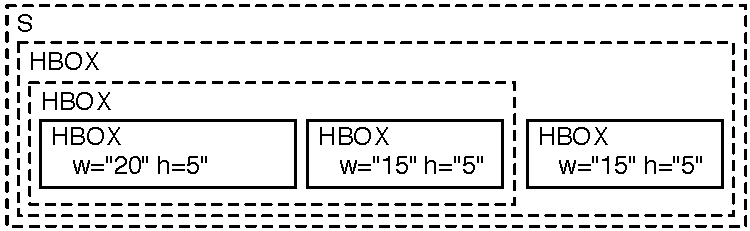
\includegraphics[trim=0 0 0 0,clip,width=1.0\columnwidth]{chapter2/output}
\end{minipage}}\\
\subfloat[\textbf{Attribute grammar for a language of horizontal boxes.}]{\label{fig:hbox:grammar}
\begin{minipage}{1\columnwidth}
\begin{grammar}
<S> \deriv{} \emph{HBOX} \\ 
  \{ HBOX.x = 0; HBOX.y = 0 \}

<HBOX> $\rightarrow$ $\epsilon$  \\
\{ HBOX.w = input$_w$(); HBOX.h = input$_h$() \} 

<HBOX$_0$> $\rightarrow$ \emph{HBOX$_1$} \emph{HBOX$_2$} \\
\{ HBOX$_1$.x = HBOX$_0$.x; \\
$~~~$ HBOX$_2$.x = HBOX$_0$.x + HBOX$_1$.w; \\
$~~~$ HBOX$_1$.y = HBOX$_0$.y; \\
$~~~$ HBOX$_2$.y = HBOX$_0$.y; \\
$~~~$ HBOX$_0$.h = max(HBOX$_1$.h, HBOX$_2$.h); \\
$~~~$ HBOX$_0$.w = HBOX$_1$.w + HBOX$_2$.w \} 
\end{grammar}
\end{minipage}
}\\
\subfloat[\textbf{Language of attribute grammars.}]{\label{fig:ag}
\usebox{\agdef}
}
\caption{For a language of horizontal boxes: (a) input tree to solve and (b) attribute grammar specifying the layout language. Specification language of attribute grammars shown in (c).%and (c) dynamic data dependencies.
}
\label{fig:hbox}
\end{figure}






\begin{figure}
\centering
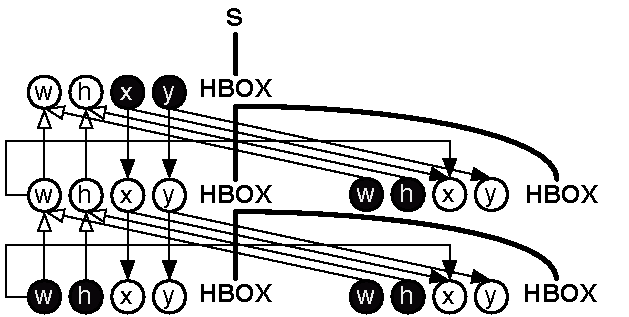
\includegraphics[trim=0 0 0 0,clip,width=0.8\columnwidth]{chapter3/deps}
\caption{\textbf{Data dependencies.} Shown for constraint tree  in Figure~2~(a). Circles denote attributes, with black circles being \sched{input()} sources. Thin lines show data dependencies and thick lines show production derivations.}
\label{fig:deps}
\end{figure}


\newsavebox{\decomplang}
\begin{lrbox}{\decomplang}% Store first listing
\begin{minipage}{1\columnwidth}
\renewcommand{\litleft}{\bfseries}
\renewcommand{\ulitleft}{\bfseries}
\renewcommand{\superscript}[1]{\ensuremath{^{\textrm{#1}}}}
\renewcommand{\subscript}[1]{\ensuremath{_{\textrm{\uppercase{#1}}}}}
\renewcommand{\syntleft}{\normalfont\itshape}
\renewcommand{\syntright}{}
\begin{grammar}
<Sched> \deriv{} \emph{Sched} ; \emph{Sched}  ~ | ~ \emph{Sched} $\vert\vert$ \emph{Sched}  ~|~ \emph{Trav}

<Trav> \deriv{} <TravAtomic> \emph{Visit}*\{(<TravAtomic> $\mapsto$ \emph{Visit}*)*\}?

<TravAtomic>  \deriv{} "parPre"  ~ | ~  "parPost"  ~ | ~  "recursive" ~ 

<Visit> \deriv{} <Prod>  \{ \emph{Step}* \}

<Step> \deriv{} \emph{Attrib} ~ | ~ "recur" \emph{V} 
\end{grammar}
%<Sched, Trav, Visit, Step> \deriv{} \ldots ~ | ~ $\hole$        
\end{minipage}
\end{lrbox}


\newsavebox{\hboxdecomp}
\begin{lrbox}{\hboxdecomp}% Store first listing
\begin{minipage}{1\columnwidth}
\begin{lstlisting}[mathescape,morekeywords={parPre,parPost}]
parPost
  HBOX$_0$ $\rightarrow$ HBOX$_1$ HBOX$_2$ { HBOX$_0$.w HBOX$_0$.h }
  HBOX $\rightarrow$ $\epsilon$ { HBOX.w HBOX.h }
;
parPre
  S $\rightarrow$ HBOX { HBOX.x HBOX.y }
  HBOX$_0$ $\rightarrow$ HBOX$_1$ HBOX$_2$ 
    { HBOX$_1$.x HBOX$_2$.x HBOX$_1$.y HBOX$_2$.y }
\end{lstlisting}
\end{minipage}
\end{lrbox}

\newsavebox{\traversals}
\begin{lrbox}{\traversals}% Store first listing
\begin{lstlisting}[mathescape,language=C++,morekeywords={spawn,join}]
void parPre(void (*visit)(Prod &), Prod &p) {
  visit(p);
  for (Prod rhs in p) 
    spawn parPre(visit, rhs);
  join;
}
void parPost(void (*visit)(Prod &), Prod &p) {
  for (Prod rhs in p) 
    spawn parPost(visit, rhs);
  join;
  visit(p);
}
\end{lstlisting}
\end{lrbox}

\newsavebox{\hboxvisitors}
\begin{lrbox}{\hboxvisitors}% Store first listing
\begin{lstlisting}[mathescape,language=C++]
void visit1 (Prod &p) {
  switch (p.type) {
    case S $\rightarrow$ HBOX:  break;
    case HBOX $\rightarrow$ $\epsilon$:
      HBOX.w = input(); HBOX.h = input(); break;
    case HBOX $\rightarrow$ HBOX$_1$ HBOX$_2$:
      HBOX$_0$.w = HBOX$_1$.w + HBOX$_2$.w;
      HBOX$_0$.h = MAX(HBOX$_1$.h, HBOX$_2$.h);
      break;
  }
}
void visit2 (Prod &p) {
  switch (p.type) {
    case S $\rightarrow$ HBOX:
      HBOX.x = input(); HBOX.y = input(); break;
    case HBOX $\rightarrow$ $\epsilon$: break;
    case HBOX $\rightarrow$ HBOX$_1$ HBOX$_2$:
      HBOX$_1$.x = HBOX$_0$.x
      HBOX$_2$.x = HBOX$_0$.x + HBOX$_1$.w;
      HBOX$_1$.y = HBOX$_0$.y
      HBOX$_2$.y = HBOX$_0$.y
      break;
  }
}
parPost(visit1, start); parPre(visit2, start);
\end{lstlisting}
\end{lrbox}


\begin{figure}
\subfloat[\textbf{One explicit parallel schedule for ~\hlang{}.}]{\label{fig:decomp} \usebox{\hboxdecomp} } \\
\subfloat[\textbf{Na\"{\i}ve traversal implementations} with Cilk's~\cite{cilk} \sched{spawn} and \sched{join}.]{\label{fig:traversals} \usebox{\traversals} } \\
\subfloat[\textbf{Scheduled and compiled layout engine for ~\hlang{}.}]{\label{fig:compiled} \usebox{\hboxvisitors} } \\
\subfloat[\textbf{Language of schedules} (without holes) ]{\label{fig:decomplang} \usebox{\decomplang} }
\caption{\textbf{Scheduled and compiled layout engine for \hlang{}.}}
\label{fig:hboxall}
\end{figure}


\begin{figure}
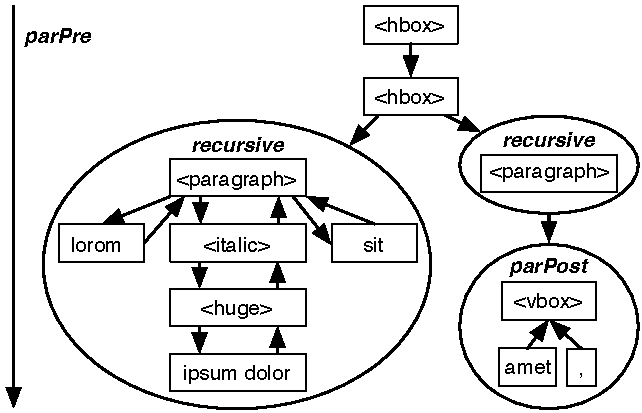
\includegraphics[trim=0 0 0 0,clip,width=1.0\columnwidth]{chapter3/nested}
\caption{\textbf{Nested traversal for line breaking}. The two paragraph are traversed in parallel as part of a preorder traversal and a sequential recursive traversal is used for words within a paragraph.}
\label{fig:nested}
\end{figure}


